%!TEX root = ../docu.tex
\section{Grundlagen}
\subsection{Mobile Anwendungen}
Software und Services können auf vershciedene wege für mobile endgeräte entwickelt und angeboten werden. Aktuelle platformen wie andorid von google oder iOS von Apple ermöglichen auf verschiedene wege das ausführen von software durch den benutzer.

hierbei haben sich zwei arten von applikationen druchgesetzt. beide bieten gewissen vor und anchteile die im folgenden näher betrachtet werden sollen.

\subsubsection{Webapplikationen}

Webapplikationen so verrät der name sind appliaktionen die über einen webbrowser auf dem gerät abgerufen werden können. deise applikationen werden von betreibern von websiten zur verfügung gestellt und laufen unabhängig der normalen webbpräsentz.

druch verschiedene kennungen kann der webserver erkennen ob besucher der webseiten von einem mobilen endgerät aus auf die zur verfügung gestellen inhalte zugreifen will und kann eine webapplikation anbieten.

diese vorm der anwendungen ist in unternehmen sehr beliebt so können verschiedene it-systeme und geshcäftsprozesse ortsunabhängig von mobilen geräten herraus gesteuern und angezeigt werden.

diese art der appliaktionen hat einen großen vorteil für die administration von mobilen endgeräten im unternhemen. so ist es möglich die isntlaltion von antiven applikationen gänzlich zuv erbeiten um sensible daten auf den gerät vor dritter zu schützen. dennoch können anwendungen über den webbrowser des geätes aufgerufen und vewendet werden.

vpn lösungen untersützen diese verfahrenweise indem sie den benutzer im unternehmens internen internet (intranet) festhalten und nur das öffnen der webappkikation im unterhmensnetzwerk erlaubt.

der sinn solcher applikatione ist neben der palttformunabhängigkeit vom betrieber eine rsparnis an zeit und ksoten für bestimtme unternehemnsprozesse.

ein beispiel sind geräte für kassensysteme in bars und restaurangs oder geräte im einsatz in algerhallen. im außendienst lösen tables und smartphones immer mehr notebooks als hauptwerkzeug der außendienstler ab. dies wird durch sinkende notekoobverkäufe auf dem bissnessektor verdeutlicht.

einige unternehmen in deutschland so z.b die RWE Gruppe führen aktionen durhc indem die mitarbeiter ihre eigenen endgeräte zur arbeit vernwende können. für diesen zweck können sie sich in das unterhemensnetzwerk verbinden und webapplikationen nutzen. diese maßnahmen sind oft mit schulen und einweißungen verbunden sollen die produktivität erhöhen ohne hohe kosten für geräte und mobilfunkverträge zu erzeugen.

\subsubsection{Native Applikationen}

native applikationen können in einer art onlineshop der jeweiligen zielplatfor erworben oder ksotenlos heruntergeladen werden. je nach plattfor varriert hier die verfahrensweise und bezahlmöglichkeit.

einmal erworbne applikationen sind dabei immer für den nutzer verfügbar. diese onlineshops bieten auch die möglichkeit bei updates der software ein upgrade der auf dem smartphone ode rtablet installierten version auf die akktuelle version.

die installierte anwendung ist nichts anderes wie eine für das jeweilige betriebsstytem geschriebene software. diese andwendung ist speziell für die palttform angepasst und entwickelt. dadurch ist der funktionsumfang der anwendung nur durch das betriebssystem begrenzt. solche anwendungen können von einen werkzeugen für das alltägliche leben bishin zu komplexen anwendungen oder sogar spielen reichen.

durch die entwicklung für die verschiedenen plattformen ist es nciht möglich z.b. eine anwendung für die iOS plattform für die android plattform zu verwenden.

es gibt dennoch anbieter solcher plattformen die die möglichkeit einräumen plattformübergreifend applikationen nutzen zu können. so ist es dem betriebssystem ubuntu phone möglich android applikationen auszuführen. diese möglichkeit wird über emulatoren realisiert. 

angebote software kann über verschiedene quellen auf das telefon gelangen. die erste ist der vom hersteller der plattform online shop welcher schon angesprochen wurde. desweiteren ist es möglich eigene software zu entwickeln und über speichermedien oder cloudspeicher uf das telefon zu übertragen und zu isntallieren.

einige herstller erlauben dieses verfahren nciht und verbieten diese möglichkeit der instlalion von nativen applikationen.

möchte ein entwicker für alle mobilen betriebssystem palttformen eine applikation anbieten ist der entwicklungsaufwand höher da für jede paltform eine native anwendung geschrieben werden muss.

alle angebotenen anwendungen müssen verschienen kriterien der jeweiligen plattformbetreeiben geprüft werden. diese technische prüfung entfällt bei installationswegen, welche vom shop abweichen. so können manuell über einen speichermedium isntalliere software nicht durch den plattformbetreiber geprüft werden.

jede auf dem ausgeführte anwendung hat theoretisch auf alle systemkomponenten des smartphones. dazu gehören unter anderem kamer speicherkarten audioeinrichtungen wie mikrofon und lautsprecher.

um die jeweiligen applikationen untereinadern zu schützen und das system als solchesslebst zu schützen wird dieses problem mit sogenanten sandboxes begegnet. die funktionsweise der sandboxen wir im kapitel \ref{sandbox} beschreiben.
\subsubsection{Verbraucher und Datenschutz}
Die isntallation von zusätzlicher software hat nicht nur vorteile sondern ermöglich es auch personenbezogene daten zu erfassen und sammeln. die unwissenheit der benutzer über die abfliesenden datenströme ist unter verbrauchen unde datenschützern viel diskutiert.

die technische unwissenheit der benutzer erleichert es  unternhemen daten von personen zu sammeln und auszuwerten. beispielsweile lassen sich ewegungsprofile erstellen und diese werdne anshcließend für gezielte werbeaktionen genutzt mit geshcäften die z.b. auf dem heimweg liegen.

der nutzer wird über die erfassung und nutzung seiner daten nicht informiert. bei der installation von software wird der bentuzer jediglich draufhingewise auf welche systemkomponenten die applikation zugreifen möchte. billigt der benutzer ein könen die anwendugen auf die komponenten jederzeit zugreifen ohne das der benutzer intervenieren kann. erst durch die deinstallation der anwendung kann die applikation keien datne mehr erfassen.

dennoch hat das sammeln von daten einen gewissen mehrwert für den benutzer. so können automatisch staumeldungen angezeigt werden, zahrzeiten zu temrinen berechnet oder die geburtstage von freunden oder verwantne geraden nciht in vergesenheit.

das unbemerkte absickern von daten ist dennoch ein probelm und wird weiterhin ein kritikpunkt bleiben.


\subsection{Die Architektur von Android}
\subsubsection{Sandboxes}
\label{sandbox}
Sandboxes ist der englishe begriff für sandkisten. olgend soll das prizip von snadboxen genauer erläutert werde. snadboxes werden häufig als sicherheits feature für andewnungen oder zum test von software verwendet.

die anwendung wird dabei vom  system auf die sie ausgeführt wird abgeschirmt und durch externe mechanismen kontrolliert. diese mechanismen stellen sicher das die anwendungen in der sandbox bleibt und regeln die informationszuführ oder den zugriffauf systemkomponnenten.

die laufende anwendung kann diese mechanismen nicht umgehen oder steuern und ist in ihrem handlungspsielraum eingeschränkt. sollte sie jedoch versuchen aus ihrem küünstlichen gefängnis herraus auzubrehcen wird dies durhc sicherungsmaßmen erkannt und ge versuch unterbrochen oder die ausführung der anwendun gänzlich gestoppt.

\begin{center}
\begin{figure}
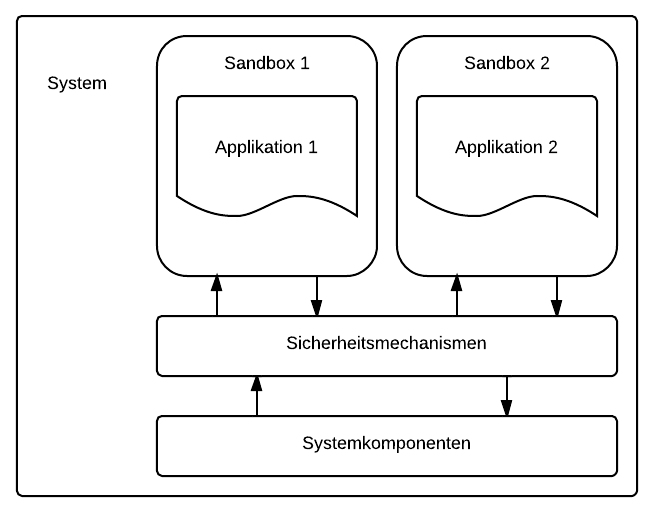
\includegraphics[scale=0.6]{images/sandbox}
\caption{Sandbox-Umgebung mit 2 Applikationen}
\label{sandbox}
\end{figure}
\end{center}

durch die verwendung von sandboxes können nicht nur test von software durchgeführt werden ohne das eigenliche system zu gefährden sodern auch anwendungen in laufzeitumgebungen ausgeführt werden um die sicherheit von daten oder dem eignetlichen system zu gewährleisten. 

auch webbrowser verwenden sandboxes für webseiten um das  system z.b. gegen die infizierung mit viren zu schützen. diese sanboxes haben auch auf vielen mobilen entgeräten ihren platz eingenommen. so werden native anwendungen auf mobiltelefonen in sandboxes ausgeführt um die anwenungen voneinander abzuschotten und um das system und ihre komponnenten zu shcützen. eine solche umgebung ist in abblidung \ref{sandbox} abstrahiert. die abbildung ezigt eine schematische darstellung eine sandbox mit appllikation.

\subsubsection{Lebenszyklus von Anwendungen}
\subsubsection{Dalvik Virtual Machine}
\subsection{Anwendungsstruktur von Android}
\subsubsection{Klassenstruktur}
\subsubsection{Berechtigungssystem}
